\begin{figure*}
    \centering
    \begin{subfigure}[b]{.39\textwidth}
        \centering
        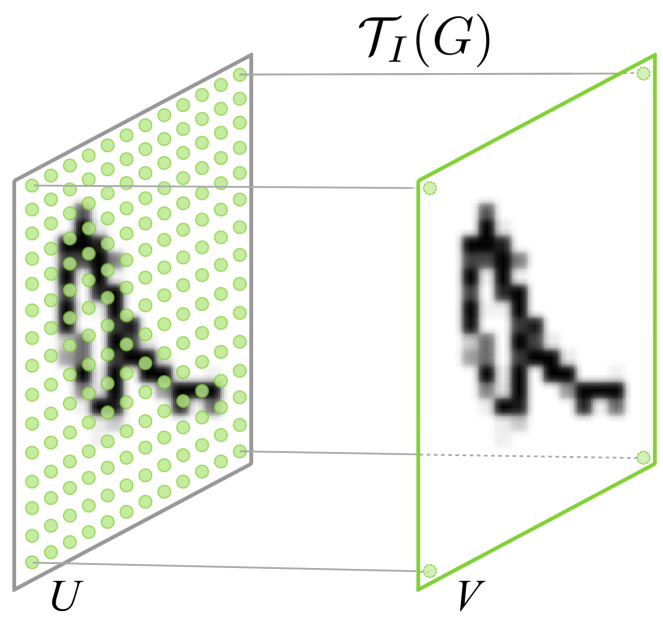
\includegraphics[width=\textwidth]{figures/neural_networks/space_transformer_ti.png}
        \caption{Sampling grid \(G' = \mathcal{T}_I(G)\) where \(I\) is the identity transformation.}\label{subfig:spacetransformer_ti}
    \end{subfigure}
    \hspace{35pt}
    \begin{subfigure}[b]{.39\textwidth}
        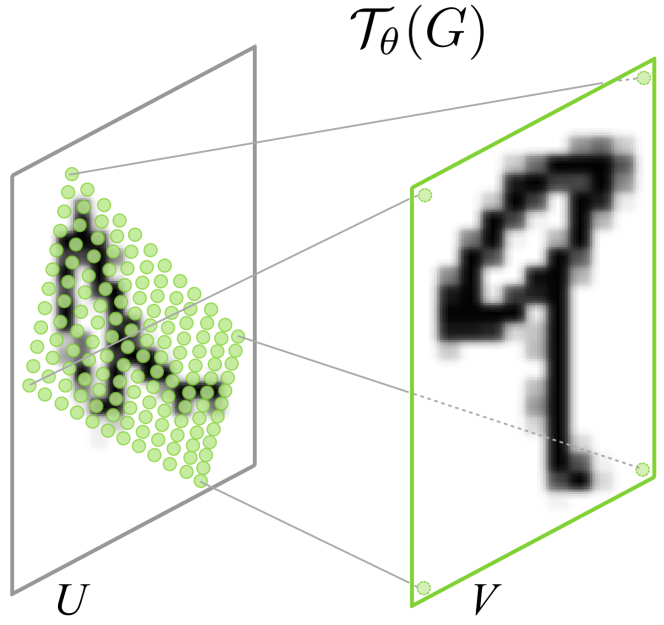
\includegraphics[width=\textwidth]{figures/neural_networks/space_transformer_ttheta.png}
        \caption{Sampling grid \(G' = \mathcal{T}_{\bm{\theta}}(G)\) where \(\bm{\theta}\) defines a 2D affine transformation.}\label{subfig:spacetransformer_ttheta}
    \end{subfigure}
    \caption{Parameterised sampling of image \(U\) to produce image \(V\) \cite{jaderberg2015spatial}.}\label{fig:paramsampling}
\end{figure*}